%%%%%%%%%%%%%%%%%%%%%%%%%%%%%%%%%%%%%%%%%
% Beamer Presentation
% LaTeX Template
% Version 1.0 (10/11/12)
%
% This template has been downloaded from:
% http://www.LaTeXTemplates.com
%
% License:
% CC BY-NC-SA 3.0 (http://creativecommons.org/licenses/by-nc-sa/3.0/)
%
%%%%%%%%%%%%%%%%%%%%%%%%%%%%%%%%%%%%%%%%%

%----------------------------------------------------------------------------------------
%	PACKAGES AND THEMES
%----------------------------------------------------------------------------------------

\documentclass{beamer}

\mode<presentation> {

% The Beamer class comes with a number of default slide themes
% which change the colors and layouts of slides. Below this is a list
% of all the themes, uncomment each in turn to see what they look like.

\usetheme{default}
%\usetheme{AnnArbor}
%\usetheme{Antibes}
%\usetheme{Bergen}
%\usetheme{Berkeley}
%\usetheme{Berlin}
%\usetheme{Boadilla}
%\usetheme{CambridgeUS}
%\usetheme{Copenhagen}
%\usetheme{Darmstadt}
%\usetheme{Dresden}
%\usetheme{Frankfurt}
%\usetheme{Goettingen}
%\usetheme{Hannover}
%\usetheme{Ilmenau}
%\usetheme{JuanLesPins}
%\usetheme{Luebeck}
%\usetheme{Madrid}
%\usetheme{Malmoe}
%\usetheme{Marburg}
%\usetheme{Montpellier}
%\usetheme{PaloAlto}
%\usetheme{Pittsburgh}
%\usetheme{Rochester}
%\usetheme{Singapore}
%\usetheme{Szeged}
%\usetheme{Warsaw}

% As well as themes, the Beamer class has a number of color themes
% for any slide theme. Uncomment each of these in turn to see how it
% changes the colors of your current slide theme.

%\usecolortheme{albatross}
%\usecolortheme{beaver}
%\usecolortheme{beetle}
%\usecolortheme{crane}
%\usecolortheme{dolphin}
%\usecolortheme{dove}
%\usecolortheme{fly}
%\usecolortheme{lily}
%\usecolortheme{orchid}
%\usecolortheme{rose}
%\usecolortheme{seagull}
%\usecolortheme{seahorse}
%\usecolortheme{whale}
%\usecolortheme{wolverine}

%\setbeamertemplate{footline} % To remove the footer line in all slides uncomment this line
\setbeamertemplate{footline}[page number] % To replace the footer line in all slides with a simple slide count uncomment this line

\setbeamertemplate{navigation symbols}{} % To remove the navigation symbols from the bottom of all slides uncomment this line
}

\usepackage{graphicx} % Allows including images
\usepackage{booktabs} % Allows the use of \toprule, \midrule and \bottomrule in tables
\usepackage[utf8]{inputenc}
\usepackage{pgfplots}
\usepackage{pifont}

\newcommand{\cmark}{{\color{green}\ding{51}}}%
\newcommand{\xmark}{{\color{red}\ding{55}}}%

%----------------------------------------------------------------------------------------
%	TITLE PAGE
%----------------------------------------------------------------------------------------

\title[CoAP]{Implementa\c{c}\~ao do protocolo CoAP para servi\c{c}os de monitoramento em Redes de Sensores Sem Fio} % The short title appears at the bottom of every slide, the full title is only on the title page

\author{Rafael de Lucena Valle} % Your name
\institute[UFSC] % Your institution as it will appear on the bottom of every slide, may be shorthand to save space
{
Universidade Federal de Santa Catarina \\ % Your institution for the title page
\medskip
\textit{rafaeldelucena@inf.ufsc.br} % Your email address
}
\date{\today} % Date, can be changed to a custom date

\begin{document}

\begin{frame}
\titlepage % Print the title page as the first slide
\end{frame}

\begin{frame}
\frametitle{Agenda} % Table of contents slide, comment this block out to remove it
\tableofcontents % Throughout your presentation, if you choose to use \section{} and \subsection{} commands, these will automatically be printed on this slide as an overview of your presentation
\end{frame}

%----------------------------------------------------------------------------------------
%	PRESENTATION SLIDES
%----------------------------------------------------------------------------------------

%------------------------------------------------
\section{Introdu\c{c}\~ao} % Sections can be created in order to organize your presentation into discrete blocks, all sections and subsections are automatically printed in the table of contents as an overview of the talk
%------------------------------------------------

\subsection{Contextualização}
\begin{frame}
\frametitle{Contextualização}

\begin{block}{Redes de sensores sem fio}
Centenas ou milhares de n\'os sensores, caracter\'isticas: pouca mem\'oria, pouco alcance do r\'adio, baixa capacidade de processamento e bateria, e custo reduzido.
\end{block}

\begin{block}{Internet das Coisas}
Objetos do cotidiano que possuem representações de seus recursos na Internet e capazes de interação com pessoas e outros objetos.
\end{block}

\begin{block}{Protocolos de aplicação}
    \begin{itemize}
        \item HTTP
        \item XMPP 
        \item MQTT
        \item \textbf{CoAP}, RFC 7252 desde 26/06/2014.
    \end{itemize}
\end{block}
\end{frame}

\subsection{Motivação}
\begin{frame}
\frametitle{Motivação}
\begin{block}{Interoperabilidade}Comunicação entre diversos dispositivos diferentes utilizando padrões.
\end{block}
    \begin{block}{Avanço Tecnológico}
        A indústria dos semicondutores e a miniaturização dos componentes.
    \end{block}
    \begin{block}{Ambientes Inteligentes}
        Novas aplicações que consumam contexto.
    \end{block}
\begin{block}{Vasta cobertura da tecnologia}
    Cerca de 5570 municípios no Brasil possuem pelo menos uma ERB.
\end{block}
\end{frame}

\subsection{Objetivos}
\begin{frame}
\frametitle{Objetivos}
\begin{block}{Objetivo Geral}
    Descrever, implementar e integrar na Internet serviços web de uma rede sensores sem fio.
\end{block}
\begin{block}{Objetivos Específicos}
\begin{itemize}
\item Portar CoAP para plataforma alvo.
\item Desenvolver a aplicação gateway GPRS / 802.15.4.
\item Desenvolver uma WEB API para coleta da informação.
\item Avaliar a solução desenvolvida.
\end{itemize}
\end{block}
\end{frame}

%------------------------------------------------

\section{Conceitos Relacionados}
\begin{frame}
\frametitle{Conceitos Relacionados}

\begin{block}{REST}
    Conjunto de princípios e restrições arquiteturais para o desenvolvimento de sistemas distribuídos.
\end{block}
\begin{block}{Restful}
    Práticas de desenvolvimento para aplicações web baseados no REST.
\end{block}
\end{frame}

%------------------------------------------------

\section{Trabalhos Relacionados}
\begin{frame}
\frametitle{Trabalhos Relacionados}
\begin{block}{Contiki}
Sistema Operacional com solução de código aberto e possui pilha IP/UDP/CoAP completa para sevidor e cliente.
Possui suporte a diversas plataformas: Econotag, OpenMote, Micaz, MSP430, ...
\end{block}

\begin{block}{OpenWSN}
Conjunto de bibliotecas de código aberto para montar uma aplicação que utilize a possui pilha IP/UDP/CoAP.
Também possui suporte a diversas plataformas: OpenMote, Zolertia Z1, WSN430, ...
\end{block}

\begin{block}{Libcoap}
Biblioteca de código aberto em C, que implementa o protocolo CoAP, que utiliza sockets POSIX.
\end{block}
\end{frame}

%------------------------------------------------

\section{CoAP}
\begin{frame}
\frametitle{Constrained Application Protocol: parte 1}
Protocolo proposto por CoRE group com as seguintes características:
\begin{itemize}
    \item Baixo overhead na validação do pacote e do cabecalho.
    \item Suporte a URI.
    \item Descoberta de recursos, GET para /well-know/core.
    \item Descoberta de serviços com socket multicast. 
    \item Protocolo desenvolvido para minimizar complexidade do mapeamento para HTTP.
\end{itemize}
\end{frame}

\begin{frame}
\frametitle{Constrained Application Protocol: parte 2}
\begin{itemize}
    \item Suporte a diferentes mídias: \textit{text/plain, charset=utf-8, application/link-format, application/xml, application/octet-stream, application/exi, application/json.}
    \item Cache simples baseado no tempo de vida (max-age) do dado captado. (opcional)
    \item Sistema de assinatura e publicação. (opcional)
    \item Confiablidade na entrega de mensagens. (opcional) 
\end{itemize}
\end{frame}

\begin{frame}
\frametitle{Constrained Application Protocol: Formato}
\begin{figure}
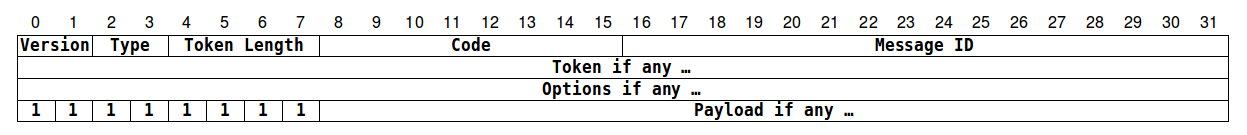
\includegraphics[width=1.0\linewidth]{../figuras/formato}
\caption{Formato do pacote em bits.}
\end{figure}
\end{frame}

\section{Implementação}

\begin{frame}
\frametitle{Implementação: Arquitetura}
\begin{figure}
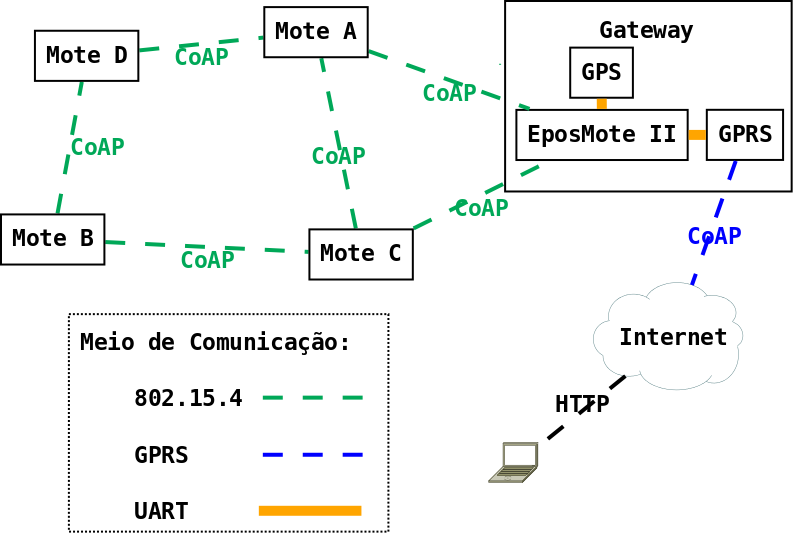
\includegraphics[width=0.9\linewidth]{../figuras/arquiteturaSlide}
\end{figure}
\end{frame}

\begin{frame}
\frametitle{Implementação: Requisitos}
Requisitos Funcionais:
\begin{itemize}
    \item Envio de requisição e recebimento de respostas CoAP.
    \item Integração com a Internet utilizando GPRS. 
\end{itemize}
Requisitos Não Funcionais:
\begin{itemize}
    \item Plataforma alvo com restrições de memória.
\end{itemize}
\end{frame}

\begin{frame}
\frametitle{Implementação: Desenvolvimento}
\begin{itemize}
    \item Levantamento de requisitos para porte de uma biblioteca CoAP. (libCoap, libCantCoap, microCoap, ...)
    \item Verificação do funcionamento da biblioteca CoAP na plataforma, utilizando testes unitários.
    \item A implementação do agendador de transmissão utiliza alarmes de disparo único.
    \item Testes de interoperabilidade utilizando exemplos funcionais (coap://coap:coap.me).
\item Gateway GPRS: ao adquirir um IP da rede, envia pacote CoAP contendo novo endereço.
\item Servidor Web: responde requisições CoAP e HTTP, envia pacotes CoAP para o gateway e mapeia os recursos CoAP para http://hostname/resources/.
\end{itemize}
\end{frame}

%------------------------------------------------
\section{Avaliação}
%------------------------------------------------

\subsection{Ambiente de Testes}
\begin{frame}
\frametitle{Ambiente de Testes: requisitos mínimos da aplicação}
Abaixo informações sobre as plataformas utilizadas para comparação.
 \begin{table}[!ht]
  \centering
  \scriptsize
  \begin{tabular}{|c|p{3cm}|p{3cm}|}
	\hline
	& \textbf{contiki/client} & \textbf{epos/client}  \\ \hline
	\textbf{Microcontrolador}	  	  & Freescale MC13224V & Freescale MC13224V \\ \hline 
	\textbf{Plataforma Alvo}    & Econotag & EposMote II\\ \hline    
	\textbf{Sistema Operacional}    & Contiki & EPOS \\ \hline    
    \textbf{Ferramentas binárias}		  & GNU Binary Utilities (2.18.50-sg++) & arm-elf-binutils 4.4.4 \\ \hline
    \textbf{Compiladores}		  & GNU C \& C++ Compilers (4.3.2-sg++) & arm-elf-g++ 4.4.4\\ \hline
    \textbf{Bibliotecas C}          & Newlib C (1.16.0-sg++) & Newlib C \\ \hline 
	\end{tabular}
  \end{table}
\end{frame}

\subsection{Resultados Experimentais}
\begin{frame}
\frametitle{Resultados Experimentais: Requisitos Mínimos}

Plataforma com 128KB Flash, 96KB RAM de memória.

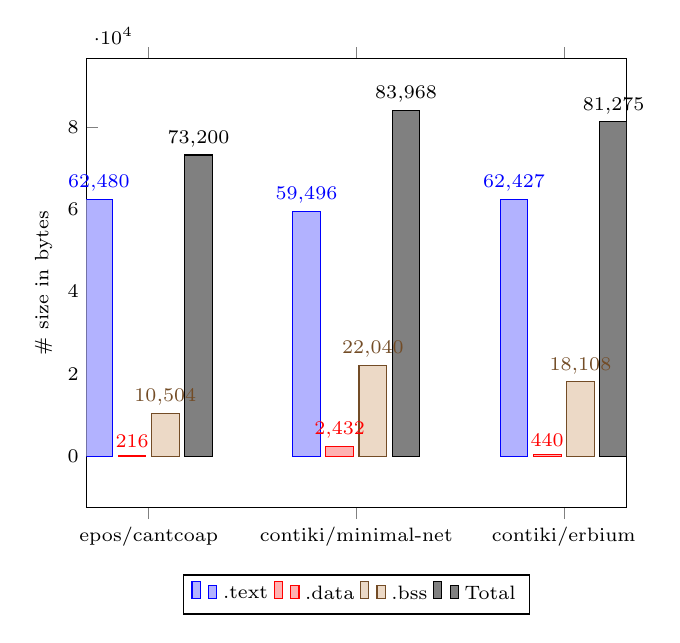
\begin{tikzpicture}
\centering
  \scriptsize
\begin{axis}[ybar , enlargelimits =0.15, legend style ={ at ={(0.5,-0.15)}, anchor =north, legend columns =-1}, ylabel ={\# size in bytes}, symbolic x coords ={epos/cantcoap,contiki/minimal-net,contiki/erbium}, xtick =data, nodes near coords , nodes near coords align ={vertical},]
\addplot coordinates {(epos/cantcoap,62480) (contiki/minimal-net,59496) (contiki/erbium,62427)};
\addplot coordinates {(epos/cantcoap,216) (contiki/minimal-net,2432) (contiki/erbium,440)};
\addplot coordinates {(epos/cantcoap,10504) (contiki/minimal-net,22040) (contiki/erbium,18108)};
\addplot coordinates {(epos/cantcoap,73200) (contiki/minimal-net,83968) (contiki/erbium,81275)};
\legend {.text,.data,.bss, Total}
\end{axis}
\end{tikzpicture}
\end{frame}

\begin{frame}
    \frametitle{Ambiente de Testes: Interoperabilidade}
    \begin{block}{Máquina Host}
     \begin{table}[!ht]
      \centering
      \scriptsize
      \begin{tabular}{|c|c|}
        \hline
        \textbf{ISA} & x86 32 \\ \hline
        \textbf{SO}	& GNU/LINUX 2.6.32-5-686 \\ \hline 
        \textbf{Distro}	& Debian 6.0.9 \\ \hline 
        \end{tabular}
      \end{table}
    \end{block}
    \begin{block}{Servidores}
    \begin{itemize}
        \item Licoap: example/etsi01.c e exemple/server.c.
        \item LibCantCoap: plain/server.c.
        \item Contiki: Erbium server e Minimal-Net server.
        \end{itemize}
    \end{block}
\end{frame}

\begin{frame}
\frametitle{Resultados Experimentais: Interoperabilidade 1}
\begin{table}[H]
\centering
\scriptsize
\label{plugTest}
\begin{tabular}{p{8cm}|c{1cm}}
\hline
\multicolumn{1}{c|}{\textbf{CEN\'ARIO}} & \multicolumn{1}{c}{\textbf{RESULTADO}} \\ \hline
\multicolumn{2}{c}{\bfseries{Testes para especifica\c{c}\~ao b\'asica CoAP}} \\ \hline
Tratar GET, confirm\'avel. & \cmark \\
Tratar POST, confirm\'avel. & \cmark \\
Tratar PUT, confirm\'avel. & \cmark \\
Tratar DELETE, confirm\'avel. & \cmark \\
Tratar GET, sem confirma\c{c}\~ao. & \cmark \\
Tratar POST, sem confirma\c{c}\~ao. & \cmark \\
Tratar PUT, sem confirma\c{c}\~ao. & \cmark \\
Tratar DELETE, sem confirma\c{c}\~ao. & \cmark \\
Tratar GET com resposta separada. & \cmark \\
Tratar requisi\c{c}\~ao com Token. & \cmark \\
Tratar requisi\c{c}\~ao sem Token. & \cmark \\
Tratar requisi\c{c}\~ao op\c{c}\~oes URI-Path. & \cmark \\
Tratar requisi\c{c}\~ao op\c{c}\~oes URI-Query. & \cmark \\
Interoperablidade em contexto de perda\\(CON mode, piggybacked response) & \cmark \\
Interoperablidade em contexto de perda\\(CON mode, delayed response) & \cmark \\
Tratar GET com resposta separada, sem confirma\c{c}\~ao. & \cmark \\ \hline
\end{tabular}
\caption{Resultados IOT Plugtest.}
\end{table}
\end{frame}

\begin{frame}
\frametitle{Resultados Experimentais: Interoperabilidade 2}
\begin{table}[H]
\centering
\scriptsize
\label{plugTest}
\begin{tabular}{p{8cm}|c{1cm}}
\hline
\multicolumn{1}{c|}{\textbf{CEN\'ARIO}} & \multicolumn{1}{c}{\textbf{RESULTADO}} \\ \hline
\multicolumn{2}{c}{\bfseries{Testes para validar o formato de dados CORE link Format}} \\ \hline
Descoberta de recursos well-known. & \xmark \\
Utiliza\c{c}\~ao de consulta para filtrar resultados. & \xmark \\ \hline
\multicolumn{2}{c}{\bfseries{Testes para validar a transfer\^encia de blocos}}\\ \hline
Transfer\^encia de blocos grandes utilizando GET (negocia\c{c}\~ao antecipada). & \xmark \\
Transfer\^encia de blocos grandes utilizando GET (negocia\c{c}\~ao atrasada). & \xmark \\
Transfer\^encia de blocos grandes utilizando o PUT. & \xmark \\
Transfer\^encia de blocos grandes utilizando o POST. & \xmark \\ \hline
\end{tabular}
\caption{Resultados IOT Plugtest.}
\end{table}
\end{frame}

\begin{frame}
\frametitle{Resultados Experimentais: Interoperabilidade 3}

\begin{table}[H]
\centering
\scriptsize
\label{plugTest}
\begin{tabular}{p{8cm}|c{1cm}}
\hline
\multicolumn{1}{c|}{\textbf{CEN\'ARIO}} & \multicolumn{1}{c}{\textbf{RESULTADO}} \\ \hline
\multicolumn{2}{c}{\bfseries{Testes para observa\c{c}\~ao de recursos}} \\ \hline
Tratar observa\c{c}\~ao de recursos. & \xmark \\
Parar a observa\c{c}\~ao de recursos. & \xmark \\
Detec\c{c}\~ao de deregistro do cliente (Max-Age). & \xmark \\
Detec\c{c}\~ao de deregistro do servidor (client OFF). & \xmark \\
Detec\c{c}\~ao de deregistro do servidor (RESET expl\'icito). & \xmark \\ \hline
\end{tabular}
\caption{Resultados IOT Plugtest.}
\end{table}
\end{frame}

\section{Conclusão}

\subsection{Conclusões}
\begin{frame}
\frametitle{Conclusões}
\begin{itemize}
    \item Foi possível a implementação de um gateway simplificado para redes de sensores sem fio e a Internet. 
    \item Desenvolveu-se uma Web API para interação com os nós. 
    \item Protocolo adequado para redes com um número grande de nós.
    \item A falta de um tipo de mídia expecífico para representação de medidas dos sensores. (SEML rascunho)
\end{itemize}
\end{frame}
\subsection{Trabalhos Futuros}
\begin{frame}
\frametitle{Trabalhos Futuros}

\begin{itemize}
    \item A implementa\c{c}\~ao da vers\~ao segura do protocolo CoAP, utilizando DLTS para comunica\c{c}\~ao segura entre os n\'os.
    \item Uma implementa\c{c}\~ao de servidor CoAP completa para executar utilizando a plataforma do EPOSMote II.
    \item Melhorar as métricas de avaliação: vazão de mensagens, round-time trip e consumo de energia e memória ao longo do tempo.

    \item Desenvolvimento de um gateway que utilize Software Defined Transceiver.

    \item Um gerador de c\'odigo que utiliza como entrada uma linguagem de especifica\c{c}\~ao dos recursos e a sa\'ida c\'odigo ANSI C m\'inimo de um servidor web utilizando CoAP e seus respectivos recursos.

    \item Modelo de apresentação de recursos para os usuários.
\end{itemize}
\end{frame}
%------------------------------------------------

\begin{frame}
\Huge{\centerline{Perguntas?}}
\end{frame}

%----------------------------------------------------------------------------------------

\end{document}
